% Created 2020-11-19 czw 09:18
% Intended LaTeX compiler: pdflatex
\documentclass[11pt]{article}
\usepackage[utf8]{inputenc}
\usepackage[T1]{fontenc}
\usepackage{graphicx}
\usepackage{grffile}
\usepackage{longtable}
\usepackage{wrapfig}
\usepackage{rotating}
\usepackage[normalem]{ulem}
\usepackage{amsmath}
\usepackage{textcomp}
\usepackage{amssymb}
\usepackage{capt-of}
\usepackage{hyperref}
\renewcommand*{\contentsname}{Spis Treści}
\usepackage[margin=3cm]{geometry}
\hypersetup{colorlinks=true,linkcolor=blue}
\usepackage{fancyhdr}
\usepackage{graphicx}
\graphicspath{ {/home/thisconnect/pwsz/} }
\pagestyle{fancyplain}
\chead{Wyszukiwanie ścieżki datagramu w internecie}
\lhead{\includegraphics{pusb.png}}
\rhead{}
\cfoot{}
\lfoot{}
\rfoot{Patryk Kaniewski \linebreak GNU GPLv3}
\author{Patryk Kaniewski}
\date{\today}
\title{Wyszukiwanie ścieżki datagramu w internecie \\
Patryk Kaniewski}
\hypersetup{
 pdfauthor={Patryk Kaniewski},
 pdftitle={Wyszukiwanie ścieżki datagramu w internecie \\
Patryk Kaniewski},
 pdfkeywords={},
 pdfsubject={},
 pdfcreator={Emacs 27.1 (Org mode 9.3)}, 
 pdflang={Polish}}
\begin{document}

\begin{titlepage}
\begin{center}
{\Huge Wyszukiwanie ścieżki datagramu w internecie \par}
\vspace{2cm}
{\Large Patryk Kaniewski \par
}\vspace{2cm}
{\large 2020-10-22}
\end{center}
\end{titlepage}
\setcounter{tocdepth}{2}
\tableofcontents \clearpage

\section{Grupa wykonująca zadanie}
\label{sec:orgcbd3574}
\begin{itemize}
\item Patryk Kaniewski
\end{itemize}

\section{Wstęp}
\label{sec:org97ad078}
\subsection{Cel ćwiczenia}
\label{sec:org3a11b9a}
Wyszukanie ścieżki datagramów w internecie
\subsection{Schemat ćwiczenia}
\label{sec:org9bb123f}
\begin{center}
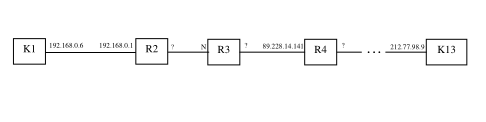
\includegraphics[width=.9\linewidth]{./schemat.png}
\end{center}
\subsection{Wymagany sprzęt}
\label{sec:org2d1170c}
\begin{itemize}
\item Komputer z systemem POSIX
\end{itemize}

\subsection{Plan ćwiczenia}
\label{sec:org99ded43}
Wybieramy cel


\subsubsection{Część 1:}
\label{sec:org61d55d1}
\begin{enumerate}
\item Pingujemy cel
\item 
\end{enumerate}



\section{Ćwiczenie}
\label{sec:org4d3434a}
\subsection{Przed ćwiczeniem}
\label{sec:orga312abf}
\subsubsection{Konfiguracja wstępna}
\label{sec:org0aec1fe}
ip a show dev enp4s0
\begin{verbatim}
2: enp4s0: <BROADCAST,MULTICAST,UP,LOWER_UP> mtu 1500 qdisc fq_codel state UP group default qlen 1000
    link/ether b4:2e:99:e4:68:04 brd ff:ff:ff:ff:ff:ff
    inet 192.168.0.186/24 brd 192.168.0.255 scope global dynamic noprefixroute enp4s0
       valid_lft 32301sec preferred_lft 32301sec
\end{verbatim}
Wybieramy cel (w moim przypadku skierniewice.eu)
\subsection{Część 1}
\label{sec:org6e8a116}
Wykonujemy ping do wybranego przez nas celu (w moim przypadku skierniewice.eu)
\begin{verbatim}
PING skierniewice.eu (94.152.194.219) 56(84) bytes of data.
64 bytes from 10.ires.pl (94.152.194.219): icmp_seq=1 ttl=55 time=7.35 ms
64 bytes from 10.ires.pl (94.152.194.219): icmp_seq=2 ttl=55 time=7.25 ms
64 bytes from 10.ires.pl (94.152.194.219): icmp_seq=3 ttl=55 time=7.26 ms
64 bytes from 10.ires.pl (94.152.194.219): icmp_seq=4 ttl=55 time=7.29 ms

--- skierniewice.eu ping statistics ---
4 packets transmitted, 4 received, 0% packet loss, time 3003ms
rtt min/avg/max/mdev = 7.249/7.285/7.345/0.038 ms
\end{verbatim}
Następnie używamy otrzymanego adresu IP do polecenia \texttt{traceroute -n 94.152.194.219} (opcja -n wyłącza odwracanie adresów ip na adresy domenowe)
\begin{verbatim}
traceroute to skierniewice.eu (94.152.194.219), 30 hops max, 60 byte packets
 1  192.168.0.1  0.227 ms  0.302 ms  0.363 ms
 2  91.214.0.129  1.521 ms  1.580 ms  1.593 ms
 3  91.214.0.1  1.595 ms  1.598 ms  1.541 ms
 4  195.43.72.106  2.128 ms  2.134 ms  2.116 ms
 5  195.182.219.60  2.583 ms  2.519 ms  2.543 ms
 6  185.80.215.238  7.068 ms  6.994 ms  7.008 ms
 7  94.152.194.219  8.233 ms !X  7.549 ms !X  7.399 ms !X
\end{verbatim}


\section{Wnioski}
\label{sec:org58a0e15}
\end{document}
